\documentclass[pdftex,12pt,a4paper]{report}

\usepackage[pdftex]{graphicx}
\usepackage{float}
\usepackage{fancyvrb}
\fvset{xleftmargin=2em}

\usepackage{pgfplots}
\pgfplotsset{width=10cm,compat=1.9}
\usepackage{tikzscale}
\usepackage{pgfplotstable}
\usepackage{booktabs}
\usepackage[font=small,labelfont=bf,tableposition=top]{caption}

\usepackage[utf8]{inputenc} % isto é um comentário
\usepackage[portuges]{babel}
\usepackage[T1]{fontenc}
\usepackage{times}
%\usepackage{lmodern}
\usepackage[obeyspaces,spaces]{url}
\usepackage[left=25mm,right=25mm,top=25mm,bottom=25mm]{geometry}
\usepackage{titlesec}
\usepackage{mathtools}
%identa 1º paragrafo de capitulos e secções
\usepackage{indentfirst}

\newcommand{\HRule}{\rule{\linewidth}{0.5mm}}
\titleformat{\chapter}{\normalfont\huge}{\thechapter.}{20pt}{\huge}


\begin{document}

\begin{titlepage}


\begin{minipage}{0.3\textwidth}
\begin{flushleft} 

\includegraphics[width=\textwidth]{./logo.png}
\end{flushleft}
\end{minipage}
\begin{minipage}{0.6\textwidth}
\begin{flushright} 

\textsc{Departamento de Engenharia Informática}\\[0.1cm]
\bfseries Mestrado Integrado em Engenharia Informática \\ [0.1cm]
\bfseries \textit{Sistemas de Representação Conhecimento e Racocínio}\\[8mm]

\end{flushright}
\end{minipage}


\vspace{3cm}


\begin{center}


\LARGE Exercício 2

\Large Extensão à Programação em Lógica e Conhecimento Imperfeito\\[1.5cm]


{\Large \bfseries Grupo 19\\[2cm] }

\begin{minipage}{0.4\textwidth}
		\large Célia Natália Lemos Figueiredo\\
           Aluna a67367
\end{minipage}
\\[1cm]
\begin{minipage}{0.4\textwidth}
		\large Gil Gonçalves \\
           Aluno a67738\\
\end{minipage}
\\[1cm]
\begin{minipage}{0.4\textwidth}
		\large José Carlos Pedrosa Lima de Faria\\
		Aluno  a67638
\end{minipage}
\\[1cm]
\begin{minipage}{0.4\textwidth}
	\large Judson Quissanga Coge Paiva\\
	Aluno  E6846
\end{minipage}


\vfill

\large Braga, {\large \today}

\end{center}
\end{titlepage}


\tableofcontents

\begin{abstract}

O presente relatório documenta o segundo trabalho prático da Unidade Curricular de Sistemas de Representação Conhecimento e Racocínio.
Nesta fase o objetivo será construir um mecanismo de representação de conhecimento com capacidade para caracterizar um universo de discurso na área da prestação de cuidados de saúde. O objetivo é demonstrar as funcionalidades subjacentes à programação em lógica estendida e à representação de conhecimento imperfeito,
recorrendo à temática dos valores nulos. Em termos gerais, foi usada a linguagem PROLOG, esta que utiliza um conjunto de fatos, predicados e regras de derivação de lógica e haverá ainda uma interação com o sistema criado para a implementação do caso prático deverá ser desenvolvida em JAVA, com recurso à biblioteca JASPER.
Neste relatório pretende-se apresentar a forma como a aplicação foi construída bem como explicar algumas decisões tomadas.


\end{abstract}
\chapter{Introdução}
\label{cap:p1}
Este primeiro capítulo tem como objetivo apresentar uma breve introdução ao exercício a realizar. Sendo assim, é necessário perceber os motivos que levaram à resolução do exercício assim como os objetivos pretendidos.
A Programação em Lógica é um tipo específico de programação cujo objetivo é a implementação de um programa cujo conteúdo se prende em factos (registos que se sabem verdadeiros), predicados (associados aos factos) e regras. A este programa podem ser estruturadas questões sobre o seu conteúdo e obter-se-ão respostas válidas e corroboradas pela lógica em si.
A programação em lógica baseia-se em dois princípios básicos para a “descoberta” das respostas (soluções) a essas questões: lógica, usada para representar os conhecimentos e informação, e Inferência, regras aplicadas à Lógica para manipular o conhecimento.

A extensão à programação em lógica surge da necessidade de abandonar conceitos restritos obrigatoriamente associados à programação em lógica abordada no primeiro trabalho prático.
A extensão à programação e lógica permite então abandonar o conceito de mundo fechado, que consiste em apenas assumir verdadeiro aquilo que se conhece (aquilo que está presente na base de conhecimento) e também abandonar o conceito de domínio fechado, que consiste em assumir que não existem mais objetos que não aqueles mencionados na base de conhecimento. Assim sendo existem, ao contrário da programação em lógica três valores de verdade, são eles os valores falso, verdadeiro e desconhecido.
Para além destas mudanças, a extensão à programação em lógica introduz o conceito de negação forte, sabendo e reconhecendo a existência da negação fraca ou negação por falha na prova (predicado não), a negação forte permite representar conhecimento negativo e é mais completa em relação à anterior pois só declara o seu valor de verdade quando de facto existe prova para tal, já a negação forte, perante falta de conhecimento considera, pelo pressuposto de mundo fechado que se este não existe então o seu valor é falso o que não é de todo correto para situações reais onde o pressuposto mundo fechado não é aplicável.
É ainda de notar que, apesar destas alterações na passagem de programação em lógica para a sua extensão os restantes conceitos mantêm-se como é o caso do pressuposto dos nomes únicos.





\section{Motivação e Objetivos}
\label{p1:MotivObj}
O PROLOG é uma linguagem declarativa, pois fornece uma descrição do problema que se pretende computar utilizando uma coleção de factos e regras lógicas que indicam como deve ser resolvido o problema proposto. Sendo também uma linguagem que é especialmente associada com a inteligência artificial e linguística computacional este é um dos grandes motivos que nos levou a querer aprender este tipo de linguagem, esta mais direcionada ao conhecimento do que aos algoritmos. 


Após os conhecimentos adquiridos na linguagem de programação lógica PROLOG, este exercício surge com o objetivo de consolidar conhecimentos e obter experiência e prática face a problemas de programação em lógica. O objetivo final será a construção de um programa capaz de armazenar conhecimento sobre registo de eventos numa instituição de saúde e através deste solucionar questões deste tema.



\section{Estrutura do documento}
\label{p1:Estrutura}
O presente relatório encontra-se organizado em cinco capítulos. Sendo que neste primeiro introduzimos a linguagem e o tema a tratar menciona-se também a motivação e os objetivos que nos levaram à realização deste exercício. 
No segundo capítulo será feito um estudo prévio da linguagem de modo a que o leitor possa entender o exercício. No terceiro capítulo explicaremos o que foi desenvolvido para a implementação do exercício. No quarto capítulo apresentaremos as conclusões e interpretação dos resultados obtidos. Por fim será apresentados um anexo com o código desenvolvido. 




\chapter{Preliminares}
\label{cap:p2}
Neste capítulo vao ser apresentados alguns conceitos fundamentais para a elaboração deste
exercício e algumas das ferramentas fundamentais para a realização do mesmo.


\section{Estudos anteriores}
\label{p2:estudp}
Para a realização deste trabalho foram necessários alguns conhecimentos anteriores sobre programação em lógica e, posteriormente, o uso da linguagem de programação PROLOG.
Este conhecimento foi adquirido ao longo das aulas teóricas ( programação em lógica) e aulas
teórico-práticas (PROLOG) de Sistemas de Representação de Conhecimento e Raciocínio.
Sobre estes conhecimentos, devemos destacar todos os conceitos que foram aprendidos tais
como o que são predicados, o que são cláusulas, o que é a base de conhecimento, entre outros
conceitos de programação em lógica que serão explicados ao longo deste documento.
Após termos alguns conhecimentos de programação em lógica falta colocá-los em prática,
e, é aqui, que entram os conhecimentos de PROLOG e da ferramenta \textit{SICSTus} usada para
compilar e interpretar o código desenvolvido nesta linguagem.
\\

Para o desenvolvimento desses predicados foi necessário fazer uma análise de conhecimentos de cada um dos membros sobre o tema e acompanhado de uma pequena pesquisa sobre as características destes.

O estudo inicial passou por caracterizar um utente, este que é definido pelo nome, serviço em que está inscrito ou consultado, profissional atribuído e a instituição onde o profissional exerce e onde o utente é atendido, que devem coincidir. Na realidade, o utente é composto por muitos outros elementos, tal como, número de utente, número de contribuinte, número de cartão de cidadão entre muitos outros, porém para simplificar e como não é necessário para este caso em estudo, vamos apenas utilizar um código e o nome do utente. 
\\




\section{Base de dados vs Representação de Conhecimento}
\label{p2:bdrepreconh}

Os sistemas de Bases de Dados (BD’s) e os sistemas de representação de conhecimento lidam
com aspectos concretos do mundo real e podem-se comparar nos termos em que dividem a
utilização da informação [Analide,2002].

Posto isto, apresentamos os pressupostos no qual se baseiam as linguagens de manipulação,
tanto das bases de dados como dos sistemas de representação de conhecimento.

\subsection{Base de Dados}
Os pressupostos em que se baseiam as linguagens de manipulação de base de dados seguem o principio de que apenas existe e é válida a informação contida nesta. Assim sendo, apresentámos
então, os seguintes pressupostos:

\begin{itemize}
	\item Pressuposto do Mundo Fechado - toda a informação não mencionada na base de dados é considerada falsa;
	\item Pressuposto dos Nomes Únicos – duas constantes diferentes ( que definam valofes atómicos ou objetos) designam, necessariamente duas entidades diferentes do universo de discurso; 
	\item Pressuposto do Domínio Fechado – não existem mais objetos no universo para além daqueles designados por constantes na base de dados.  
\end{itemize}

\subsection{Sistema de Representação de Conhecimento}


Porém, nem sempre se pretende assumir que a informação representada é a única que se pode
considerar válida e que as entidades representadas sejam as únicas existentes. Posto isto, apresentámos, então, os seguintes pressupostos:

\begin{itemize}
	\item Pressuposto do Mundo Aberto - podem existir outros factos ou conclusões verdadeiros para além daqueles representados na base de conhecimento; 
	\item Pressuposto dos Nomes Únicos – duas constantes diferentes ( que definam valores atómicos ou objetos) designam, necessariamente duas entidades diferentes do universo de discurso; 
	\item Pressuposto do Domínio Aberto – podem existem mais objetos do universo de discurso para além daqueles designados pelas constantes da base de conhecimento.  
\end{itemize}

\section{Representação da Informação Incompleta}


Muitas vezes presenciámos situações onde a informação existente é insuficiente e/ou incompleta.
Perante estas situações, é importante saber representá-las para além do verdadeiro ou
falso; temos de ser capazes de demonstrar que a questão/situação em causa é incompleta/desconhecida
e que o seu valor não pode ser definido no imediato, ao contrário do que acontece,
na maior parte das situações, nas mais variadas linguagens de programação.
E aqui que a programação em lógica estendida se apresenta como capaz de resolver estas
situações. Através da programação em lógica estendida seremos capazes de representar tais
situações desconhecidas. A forma de representar o conhecimento é apresentada a seguir:


\begin{itemize}
	\item Verdadeiro: quando for possivel provar uma questão(Q) na base de conhecimento; 
	\item Falso: quando for possível provar a falsidade de uma questão(-Q) na base de conhecimento;
	\item Desconhecido: quando não for possível provar a questãoQ nem a questão-Q
\end{itemize}


De facto, para cumprir com os pressupostos definidos anteriormente, teremos de definir outro tipo de informação, além da informação positiva e a informação negativa. Esta pode ser
representada da seguinte forma:


\begin{itemize}
	\item Negação por Falha: quando não existe nenhuma prova. É representada pelo teorema \textit{não}, anteriormente utilizado no \textit{Exercício 1};
	\item Negação Forte:  representada por (-) e que afirma que determinado predicado é falso.
\end{itemize}

Por fim, atendendo aos requisitos do trabalho, será ainda necessário obdecer às seguintes
caracteristicas:

\begin{itemize}
	\item Representar casos de conhecimento imperfeito, pela utilização de valores nulos de todos os tipos estudados;
	\item Manipular invariantes que designem restrições de inserção e remoção de conhecimento do sistema; 
	\item Lidar com a problemática da evolução do conhecimento, criando os procedimentos adequados;
	\item Desenvolver um sistema de inferência capaz de implementar os mecanismos de raciocínio inerentes a estes sistemas.

\end{itemize}

\chapter{Descrição do Trabalho e Análise de Resultados}
\label{cap:p3}

Nesta parte do documento serão explicitadas todas as etapas de resolução dos desafios fornecidos bem como todas as decisões efetuadas no processo.


\section{Base de Conhecimento}
\label{p3:baseConhe}

A base de Conhecimento define bases de dados ou conhecimento acumulados sobre determinado assunto.
Para a elaboração deste exercício tornou-se importante definir uma base de conhecimento
que possa responder aos pedidos do enunciado.

\section{Funcionalidades Básicas}
\label{p3:funcbasic}
Nesta secção serão apresentados e explicados os métodos usados para a resolução das funcionalidades básicas propostas.

\subsection{Representação de Conhecimento Positivo e Negativo}

A representação do conhecimento positivo é feito nos factos, por exemplo:


\subsection{Representação de casos de Conhecimento Imperfeito, pela utilização de valores nulos de todos os tipos}



\subsection{Manipulação de Invariantes que designem restrições à inserção e à remoção de conhecimento}


\subsection{Tratamento de problemática da evolução do conhecimento, pela criação dos procediemntos adequados}


\subsection{Desenvolvimento de um sistema de inferência capaz de implementar os mecanismos de raciocínio inerentes a estes sistemas}

\begin{figure}[<+htpb+>]
	\centering
	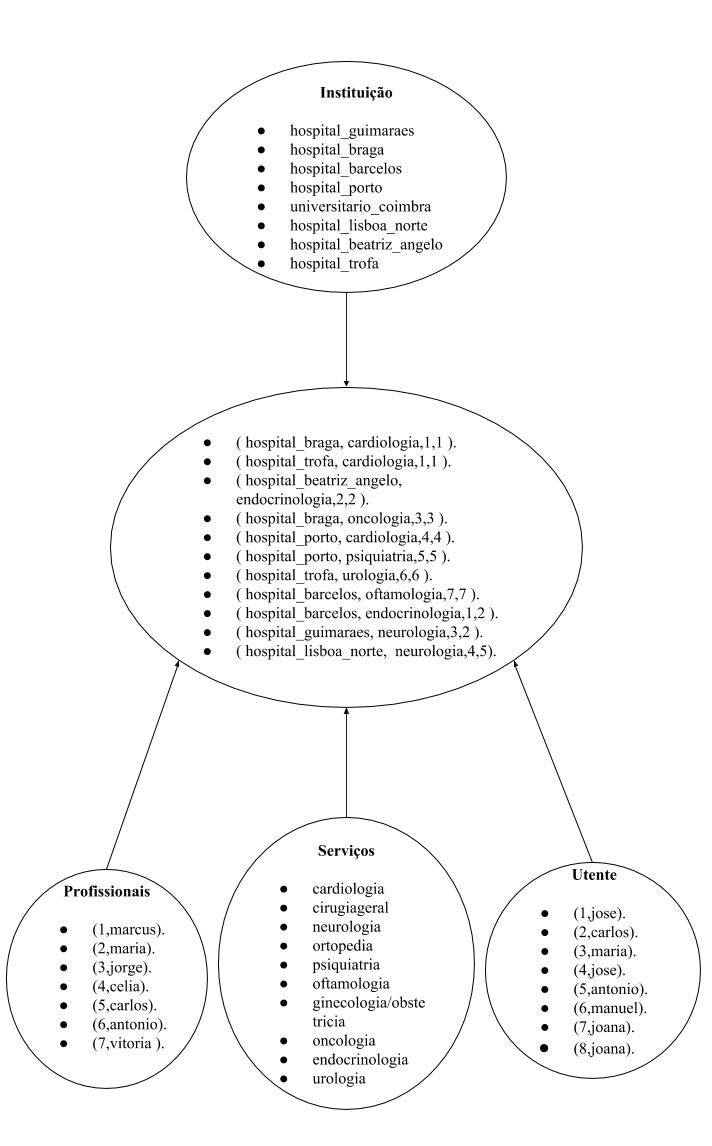
\includegraphics[scale=0.18]{esquema.jpg}
	\caption{Esquema da base de conhecimento }
	\label{p3:fig:esquema1}
\end{figure}





\chapter{Conclusão}

O trabalho apresentado cumpre todos os requisitos propostos.
Foi feito um gerador de figuras com capacidade de gerar pontos para um plano, caixa, cone e esfera como pedido. Além destas figuras foram ainda desenvolvidas funções adicionais que permitem criar planos sem ser no eixo XZ bem como foram desenvolvidas funções para a criação de círculos e cilindros, algo que não era expressamente pedido.

No lado do motor, a aplicação consegue ler ficheiros XML e .3D e a partir dai desenhar as figuras com os pontos especificados nos ficheiros. Adicionalmente ao sugerido, incluiu-se também uma câmara colocada sobre uma esfera que permite ao utilizador ver a figura desenhada de vários ângulos. Incluiu-se ainda um pequeno menu para alterar o modo de visualização da figura.

O código produzido recorreu ao uso de classes, o que evitou bastantes repetições de código e sobretudo gerou um código fácil de ler, perceber e manter. Por estes motivos, considera-se como bastante sólido o trabalho desenvolvido.

Não obstante, existem aspectos em que o trabalho que poderiam ser melhorados e serão alvo de atenção no futuro. 

Em primeiro lugar, destaca-se a questão da câmara. Nesta fase implementou-se a câmara usando coordenadas esféricas. Decidiu-se que a camâra seria por isso apenas uma instância da classe \textit{CoordsEsfericas}. Deste modo mover a câmara corresponde apenas a chamar as funções definidas na classe. Este aspecto facilitou imenso a implementação da câmara, no entanto trouxe também algumas desvantagens. Sendo a câmara uma instância de \textit{CoordsEsfericas} significa que a câmara só pode ter coordenadas esféricas. Isto dificulta a adição de funcionalidades extra à câmara. Além disso, enquanto que é perfeitamente válido que as coordenadas esféricas possam referir um ponto ``no polo norte'' da esfera, tal não é verdade para a câmara, pois nesse caso o objeto pode deixar de se tornar visível. Isto deixa a entender que no futuro a câmara terá que pertencer a uma classe própria e muito provavelmente será esse o caminho a seguir.

Em segundo lugar, refere-se a modularidade e encapsulamento de dados, aspectos que foram deixados um pouco para segundo plano. A prioridade desde cedo foi ter código simples, funcional e fácil de ler. Tal implicou que muitas vezes quando confrontados com a decisão de manter algumas variáveis como públicas ou privadas a decisão tenha sido manter públicas. Exemplos disso são as classes Ponto3D (note-se a falta de getters e setters) e as classes das coordenadas esféricas e polares. Enquanto que ter variáveis públicas em classes como a Ponto3D seja relativamente irrelevante, tal já não é verdade para as classes das coordenadas. Como o objetivo principal do projeto não é ter bons módulos de dados nem bom encapsulamento dos mesmos, estes aspectos foram deixados para segundo plano, no entanto serão alvo de uma atenção mais cuidada no futuro.

\end {document}